\chapter*{Schedule revision}
\addcontentsline{toc}{chapter}{Schedule revision}
\label{chap:schedule-revision}
As we said before, and once our knowledge of Bitcoin arrived at a low-level detail, we realized the time we estimated for script and transaction modelling was too optimistic so changes appeared in the planning from that task forward.
\section{Changes motivation}
As appears in the previous methodology chapter, we'll dedicate more time to transaction modelling and script creation and to its testing and try to reduce the implementation time as with the framework created it will suppose to be simple and not require much lines of code. This way we want to achieve the goal by redistributing the time assigned to its task.
\section{Other minor changes}
In order to make the Gantt diagram simpler, we've reduced the iteration to design, implement, test and launch that mean to create, implement, test and broadcast transactions respectively. Therefore it's understood that in each iteration cycle, a different transaction will be developed, requiring 3 transactions modelling per channel (and that the unidirectional channel has to be implemented). Also several subtasks were reduced to a main task to reduce the resulting Gantt diagram size and iterations were defined to fullfill all diagram time lapse.
\clearpage
\section{Resulting Gantt diagram}
After performing the previously mentioned changes, we obtain the following new Gantt diagram:
\begin{figure}[ht]
  \centering
  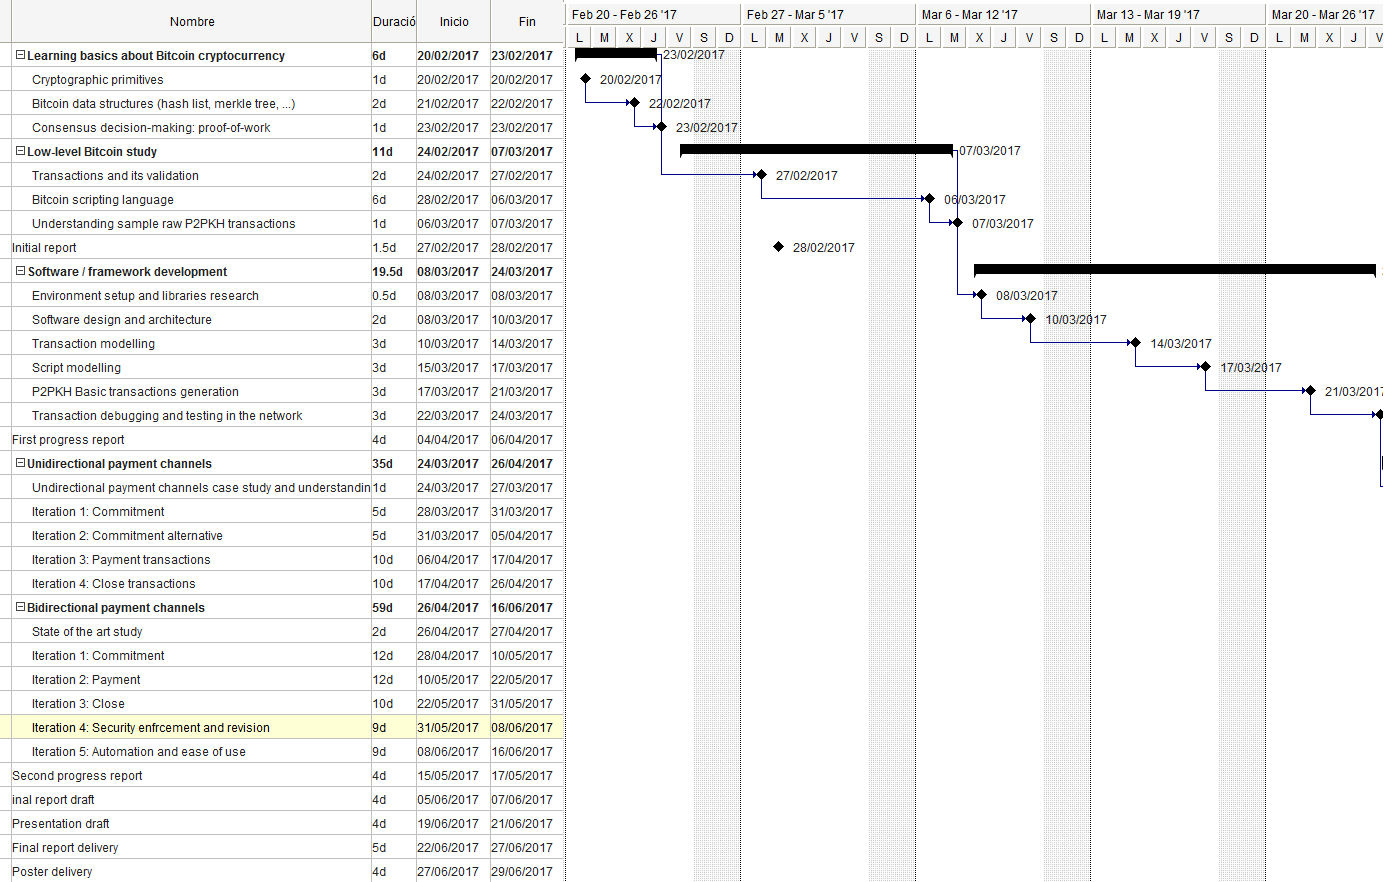
\includegraphics[width=\linewidth]{tasks-feb-mar}
  \caption{Gantt diagram of the new schedule [February-March]}
  \label{fig:gantt-diagram-feb-mar}
\end{figure}
\begin{figure}[ht]
  \centering
  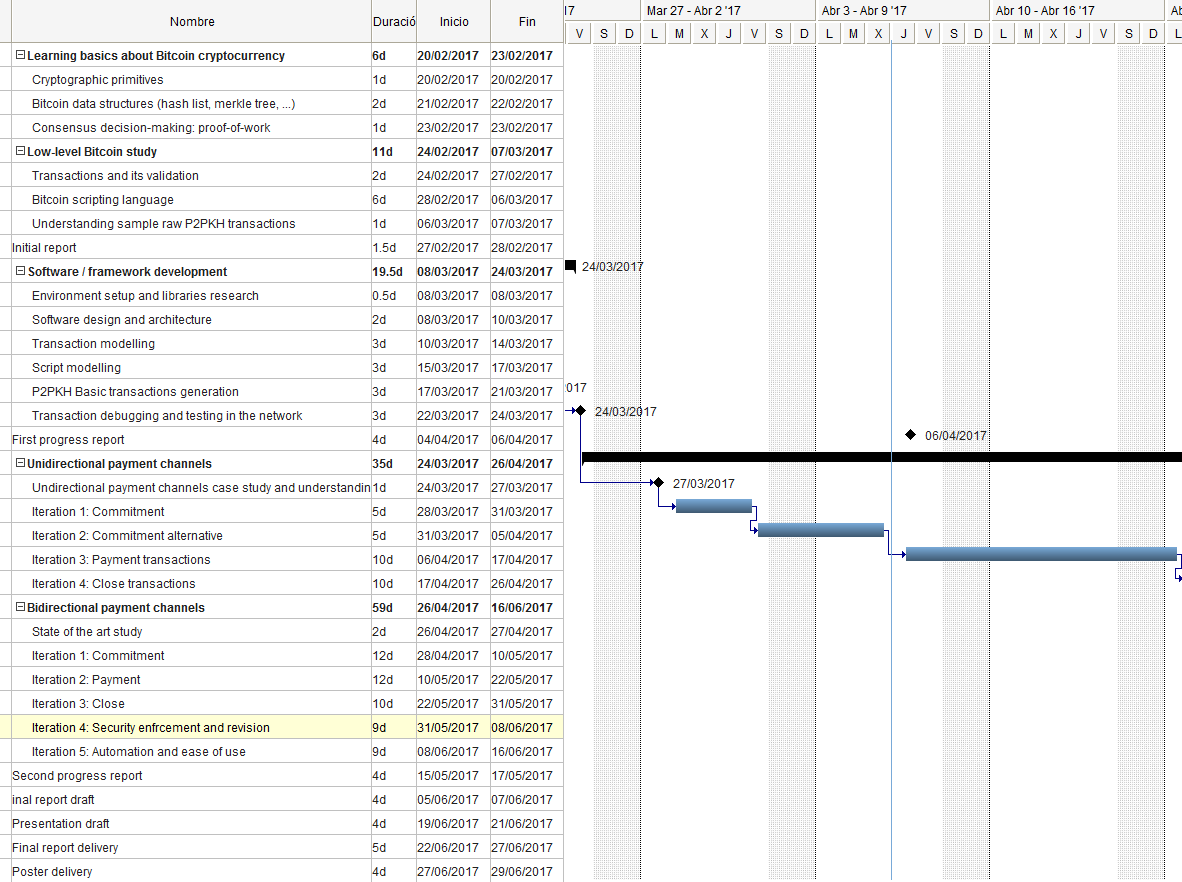
\includegraphics[width=\linewidth]{tasks-mar-apr}
  \caption{Gantt diagram of the new schedule [March - April]}
  \label{fig:gantt-diagram-mar-apr}
\end{figure}
\begin{figure}[ht]
  \centering
  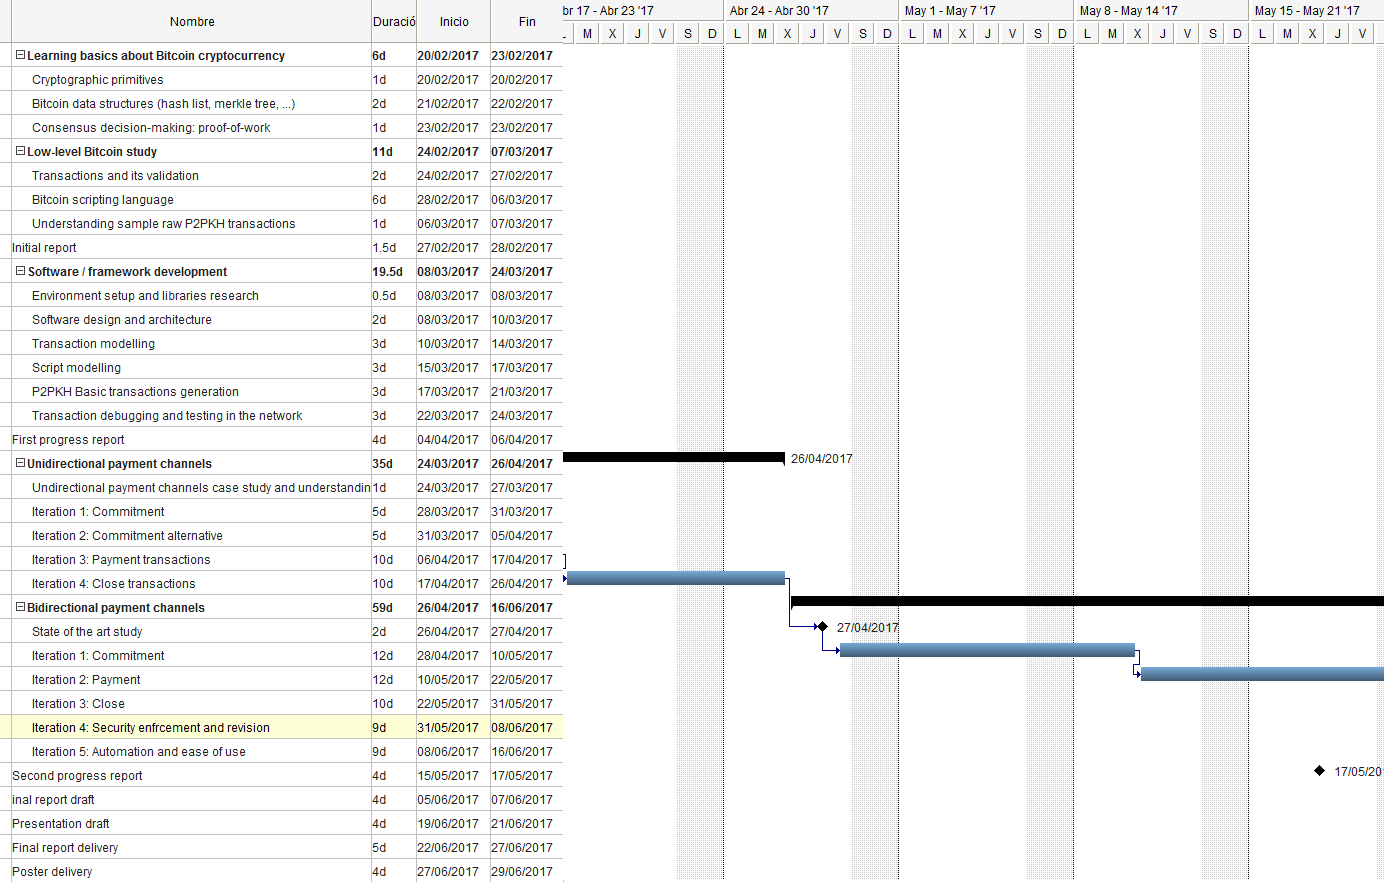
\includegraphics[width=\linewidth]{tasks-apr-may}
  \caption{Gantt diagram of the new schedule [April - May]}
  \label{fig:gantt-diagram-apr-may}
\end{figure}
\begin{figure}[ht]
  \centering
  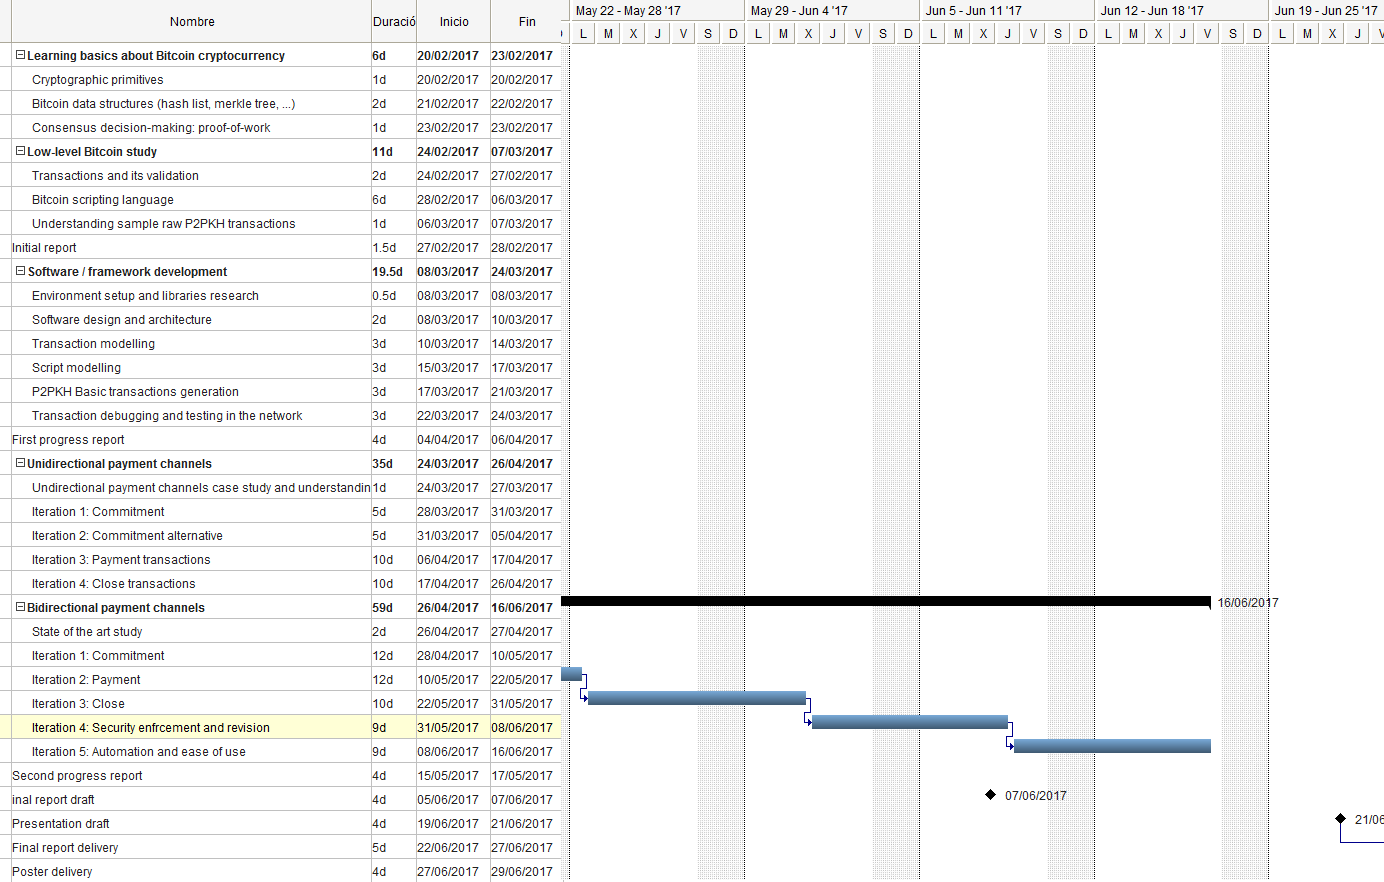
\includegraphics[width=\linewidth]{tasks-may-jun}
  \caption{Gantt diagram of the new schedule [May - June]}
  \label{fig:gantt-diagram-may-jun}
\end{figure}
\begin{figure}[ht]
  \centering
  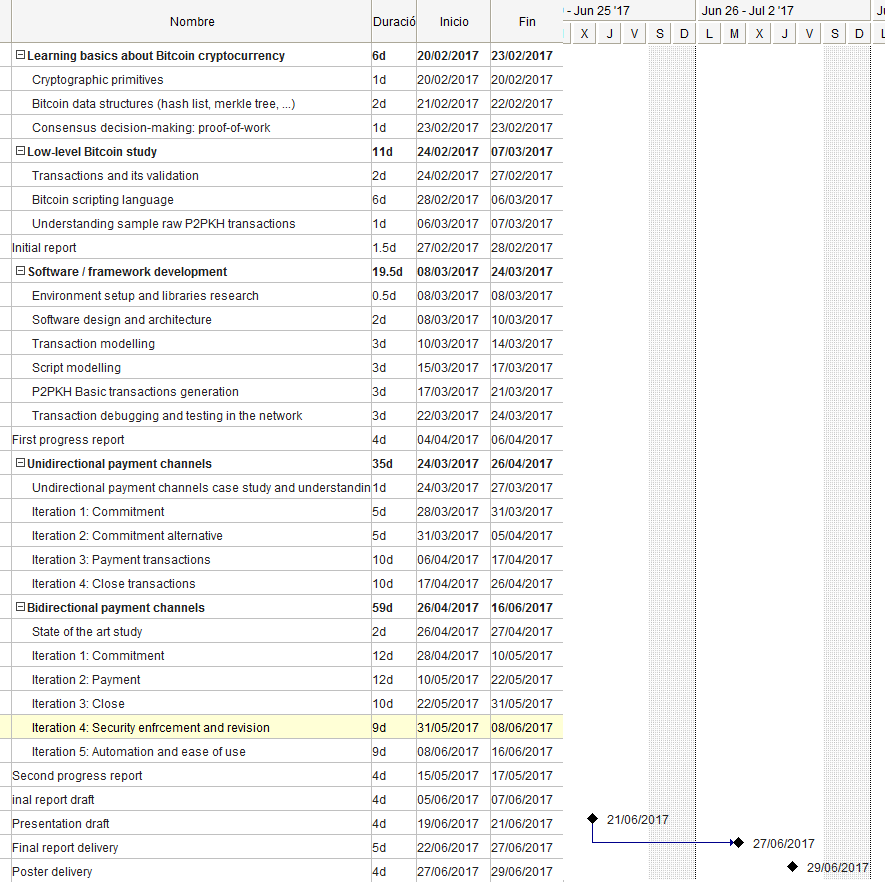
\includegraphics[width=\linewidth]{tasks-end}
  \caption{Gantt diagram of the new schedule [June - end]}
  \label{fig:gantt-diagram-end}
\end{figure}